\renewcommand{\arraystretch}{1.5}
\textbf{Induktionsgesetz}\\
		\begin{tabular}[c]{p{8.7cm}}
			$u_i= \mp \dot{\Phi} = \mp \frac{d}{dt} \int \vec{B} \cdot
			\vec{dA}\qquad $ \parbox{3cm}{\tiny{$- \Rightarrow B,u_i $
			Rechtsschraube\\ $+ \Rightarrow B,u_i $
			Linksschraube}}
			\\
			
			$u_i= \mp \dot{\Psi}\qquad$ , meist $\; u_i = \mp
			N\cdot\dot{\Phi}$		
		\end{tabular}
		\parbox{8cm}{Durchsetzt das sich \"andernde Magnetfeld einer stromdurchflossenen Spule
					eine zweite Spule, so wird auch in dieser eine Spannung
					(=Gegeninduktionsspannung) induziert.}	

\begin{multicols}{2}
 		\textbf{Gegeninduktion} ($M_{\textcolor{blue}{X}\textcolor{orange}{Y}}; \textcolor{blue}{X}$: Wirkung,
 		$\textcolor{orange}{Y}$: Ursache)\\
		\begin{tabular}{ll}
  		Gegeninduktivit\"at
  			& $M_{21} = \frac{\Psi_{m21}}{i_1}$ Meist $= \frac{N_2 \phi_{m21}}{i_1}$\\ 
  			(wenn $\mu$ = const.) & $M = k \cdot \sqrt{L_1 L_2} = M_{21} = M_{12} $  \\
  			Gegeninduktionsspannung
  			& $u_{21} = \dot{\Psi}_{21} = M_{21} \frac{di_1}{dt}$ \\
		\end{tabular}\\

  		\textbf{Transformatorgleichungen}\\
		$\boxed{u_1 = L_1 \dfrac{di_1}{dt} \textcolor{red}{+}\textcolor{green}{-}M_{12}
		\dfrac{di_2}{dt} = L_1 \dfrac{di_1}{dt} \textcolor{red}{-}\textcolor{green}{+}M_{12} \dfrac{di_b}{dt}}$ \\
		$\boxed{u_2 = L_2 \dfrac{di_2}{dt}\textcolor{red}{+}\textcolor{green}{-} M_{21}
		\dfrac{d i_1}{dt} = -L_2 \dfrac{di_b}{dt}
		\textcolor{red}{+}\textcolor{green}{-} M_{21} \dfrac{d i_1}{dt}}$\\
		Im Bildbereich:\\
		$\underline{U}_1 = j\omega\cdot L_1 \cdot \underline{I}_1 + j\omega\cdot M \cdot \underline{I}_2$\\
		$\underline{U}_2 = j\omega\cdot L_2 \cdot \underline{I}_2 + j\omega\cdot M \cdot \underline{I}_1$\\
  			
	  	\textbf{Idealer Trafo}\\ 
	  	$"u = \dfrac{u_1}{u_2} = \dfrac{N_1}{N_2} = \sqrt{\dfrac{L_1}{L_2}}$ $\qquad$ (im Leerlauf:
	  	$\dfrac{1}{"u} = k \sqrt{\dfrac{L_2}{L_1}}$)\\

  		\textbf{Verlustbehafteter Trafo}
  		\begin{list}{$\bullet$}{\setlength{\itemsep}{0cm} \setlength{\parsep}{0cm} \setlength{\topsep}{0cm}} 
          \item Prim\"arstrom im Leerlauf: $L_H$
          	(ideal $L_H \rightarrow \infty)$
          \item Hysterese- \& Wirbelstromverluste: $R_{Fe}$ \newline
          	(ideal: $R_{Fe}\rightarrow \infty$) 
          \item Kupferwiderst\"ande: $R_{Cu1}, R_{Cu2}$
          	(ideal: $R_{Cu}
          \rightarrow 0$)
          \item Streufluss (Kopplung): $L_{\sigma1}, L_{\sigma2}$
          	(ideal: $L_{\sigma} \rightarrow 0$)
        \end{list}

	\columnbreak
  		\begin{flushleft}
  		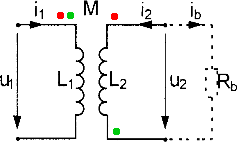
\includegraphics[width=4cm]{bilder/trafo-kopplung.png} \\
  		\small{\textcolor{red}{Gleichsinnig} / \textcolor{green}{Gegensinnig}} \\
  		\vspace{1cm}

	  	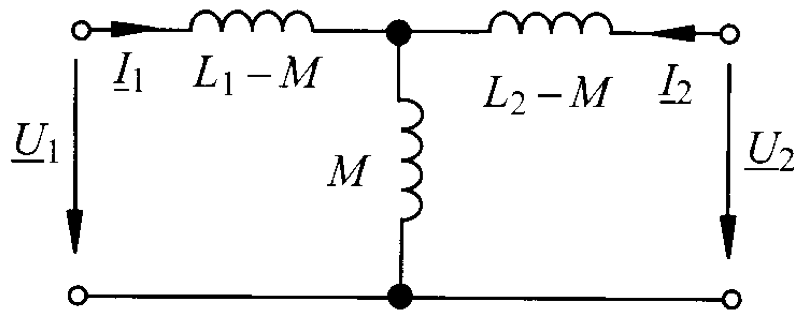
\includegraphics[width=5cm]{bilder/T_Ersatzschaltbild_VST.png}\\
		\end{flushleft}  	
	
\end{multicols}
\renewcommand{\arraystretch}{1}